
% new
\section{3D Environments}\label{chap2:3denvironment}

\begin{figure}[!ht]
    \centering
    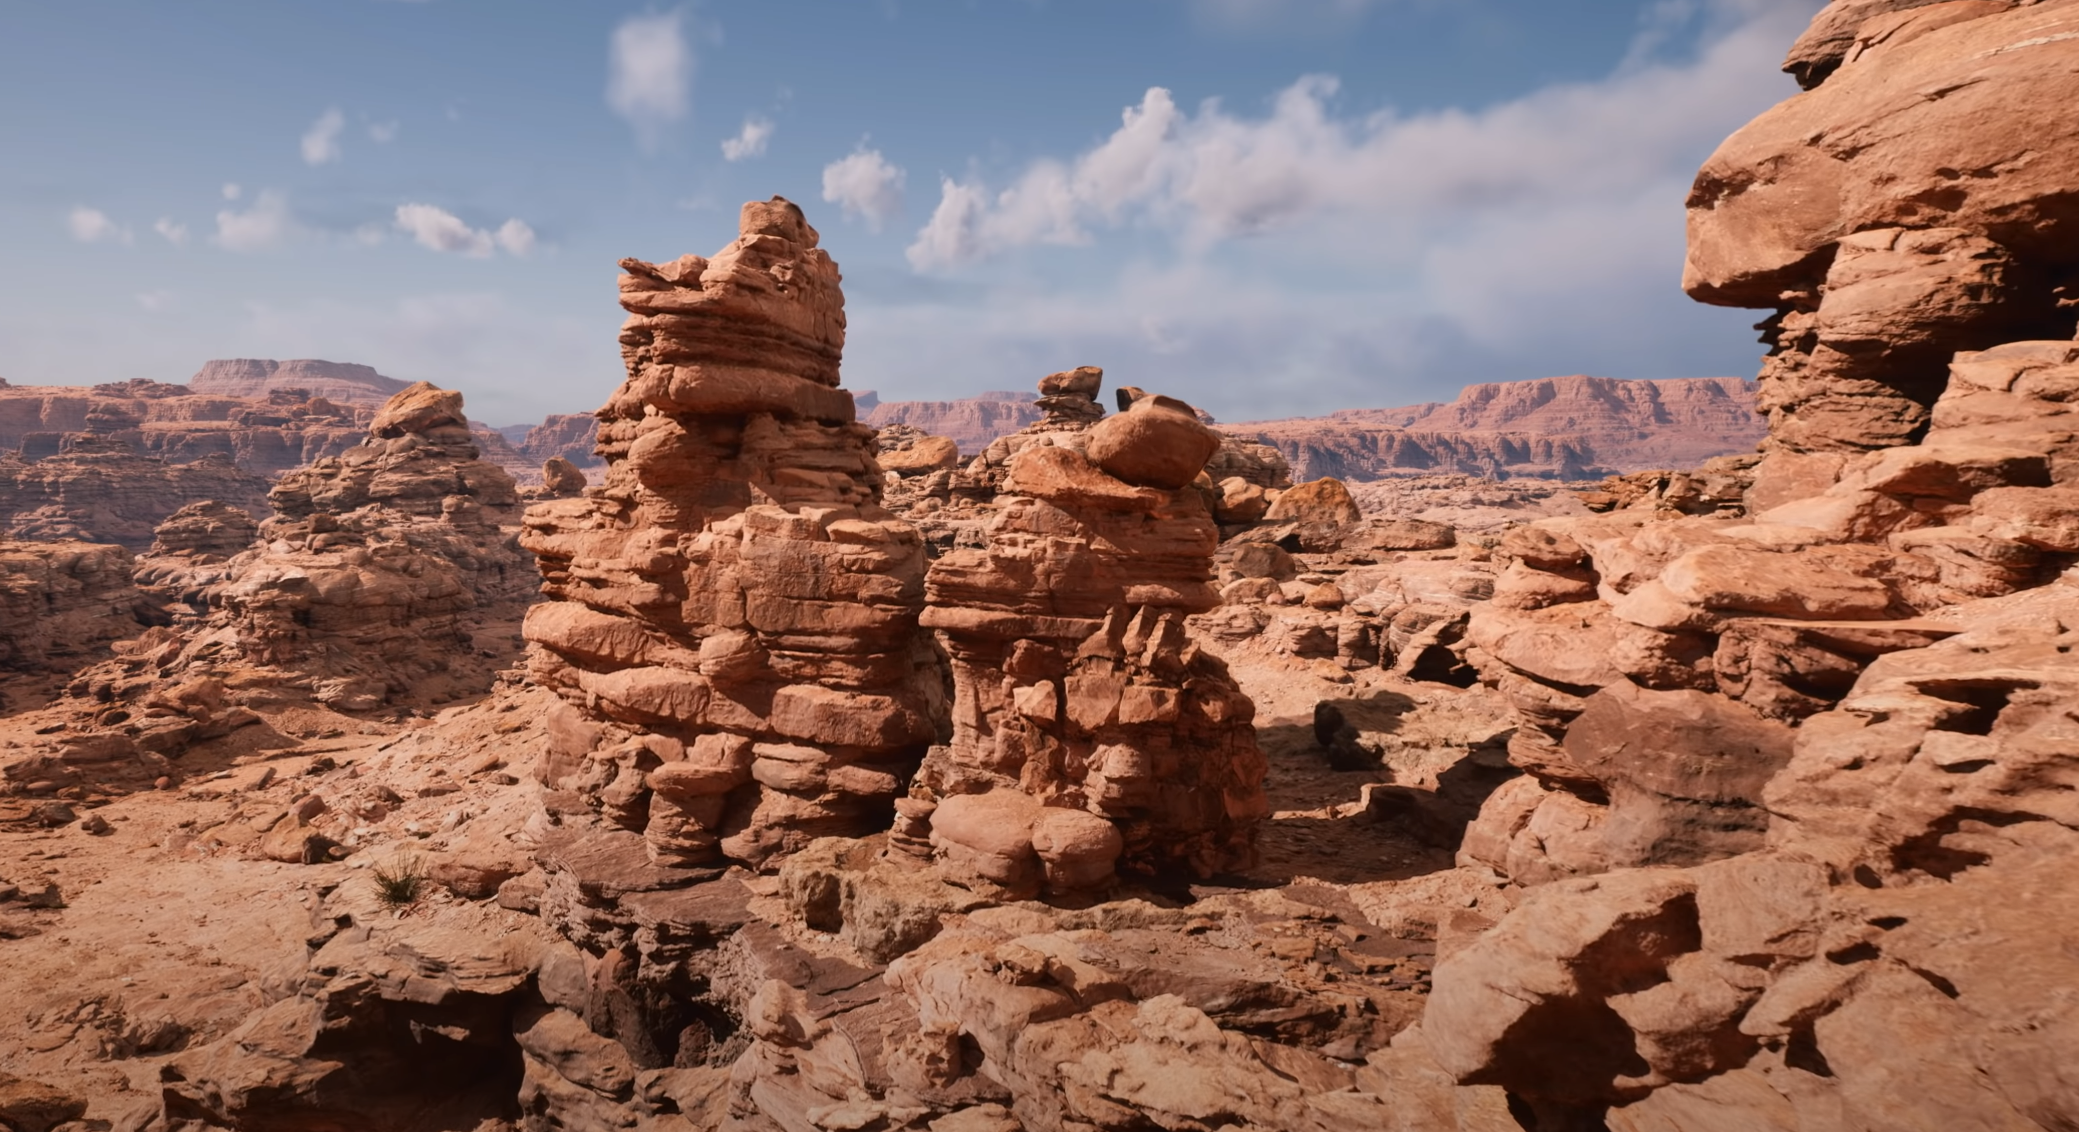
\includegraphics[width=0.7\textwidth]{images/unreal-desert2.png}
    \caption{3D hyper-realistic simulated desert using Unreal Engine 5 (early access) \cite{unreal5_2021}.}
    \label{fig:unreal-desert}
\end{figure}
    
    
Current software allows the creative development of simulated 3D environments, which can be executed and visualized on a variety of platforms, such as smartphones, gaming consoles, etc. 
% These 3D environments 
% https://spatial.io/
It is remarkable how the applications of simulated hyperrealistic environments continue to grow every year in architectural renderings, advertisements of specialized computer software, video games, movies, video calls \cite{spatial-io2021}, etc.
% overall creating a more immersive experience across all domains, where realism in 3D modeling software and game engines continues to improve.
The advent of 3D computer graphics, GPUs, rendering engines and techniques, and game engines continue to allow developers to come up with more sophisticated world simulations.
Life-like simulations are therefore possible through 3D environment modeling \cite{asma_2021}, which involves steps such as:
% source https://it-s.com/what-is-a-3d-modeled-environment/
\begin{enumerate}
    \item \textbf{Detailed concept development} of blueprints and insight of state-of-the-art art techniques
    \item \textbf{High-definition sketching} based on the predefined concepts 
    \item \textbf{Environment assets creation} of the objects that will be in the scene
    \item \textbf{Hyper-focused texturing} of the given objects, where natural textures must be applied to allow realism under different perspectives and lighting conditions.
    \item \textbf{High/Low-Poly modeling} depending on the purpose of the project and hardware constraints for rendering (real-time factor).
    \item \textbf{3D rendering and optimization} of parameters and light settings.
\end{enumerate}

The following sections give a brief overview of what game engines are and how they enable the creation of synthetic data for machine learning models.

\subsection{Game Engines and Simulation Environments}\label{chap2:gameengines}
Game Engines, like integrated development environments (IDEs), are software frameworks that allow the development of video games and 3D environments by providing an abstraction layer over a multitude of functionalities. They consist of a main game program, a rendering engine, an audio engine, a physics engine, and an artificial intelligence module, which take care of the following: 
\begin{itemize}
    \item \textbf{Input} from a multitude of devices such as keyboards, mice, screens, etc. This input can be obtained through polling or event-based mechanisms (i.e., obtaining the position of a cursor is polling-based and detecting a click from a mouse is event-based).
    \item \textbf{Graphics} which are generated by converting the geometric and color information of a scene from the virtual space of the application into a picture. This requires the usage of 3D assets, which are usually created using 3D modeling software such as Blender, Autodesk 3ds Max, Maya, etc. 
    \item \textbf{Physics}, where the laws of gravity, friction, and collision for the movement of a virtual object are simulated.
    \item \textbf{Artificial Intelligence} to give the characters in the environment a personality, such as animals, etc.
    \item \textbf{Sound} to represent sound effects, dialogue, music, etc. 
    \item \textbf{Networking} to abstract TCP/UDP and API integrations in the development of multiplayer games.
\end{itemize}

Physics simulators are an important part of robotics research, as they provide an environment for researchers to test and evaluate algorithms and/or architectures without the constraints and real-world complexity of the physical environment, including the physical degradation of robots. When simulating robots, one of the first questions we need to ask is what level of complexity we are willing to tackle, and where the simulations are going to be used. Moreover, simulations can run faster than real time, are parallelisable, and allow the environment to be reset or modified without physical effort. Finally, simulations are able to produce different sensory inputs which can be extremely valuable for robotics research.

\textcite{collins2021review} define a robotics simulator as an end-user software application that contains a realistic physics engine, collision and friction detection, GUI, supports 3D assets, allows a scripting mechanism, and can model robotic joints and actuators. Relevant game engines and simulation environments that can be used in the development of machine learning or robotic applications include: Unity 3D \cite{unity2021}, Unreal Engine \cite{unreal5_2021}, MuJoCo \cite{mujoco}, Gazebo Simulator \cite{osrf2021gazebosim} and CARLA \cite{Dosovitskiy17}.
% An overview of these frameworks is described below.
% \textbf{Unity 3D.}\label{chap:2:unity}
\textcite{collins2021review} provide an in-depth review of physics simulators for robotics applications with extensive comparative tables that set one simulator apart from other for each use case. Factors taken into account in the evaluation of the simulators include: fidelity of rigid or soft body contact dynamics, locomotion over irregular terrain, support for torque and vision sensors, noise simulation in sensors to approximate real world policies, domain randomization to diversify training data, texture randomization, randomization of object mass, inertia, and friction coefficients, support for multiple physics engines, support for parallel simulation, support for headless mode and rapid dynamic solvers, support for CPU and GPU optimizations.
% \begin{itemize}
%     \item Fidelity of rigid or soft body contact dynamics.
%     \item Locomotion over irregular terrain.
%     \item Support for torque and vision sensors, among others.
%     \item Noise simulation in sensors to approximate real world policies.
%     \item Domain randomization to diversify training data.
%     \item Texture randomization.
%     \item Randomization of object mass, inertia, and friction coefficients.
%     \item Support for multiple physics engines.
%     \item Support for parallel simulation.
%     \item Support for headless mode and rapid dynamic solvers.
%     \item Support for CPU and GPU optimizations.
% \end{itemize}

\begin{figure}[!ht]
    \centering
    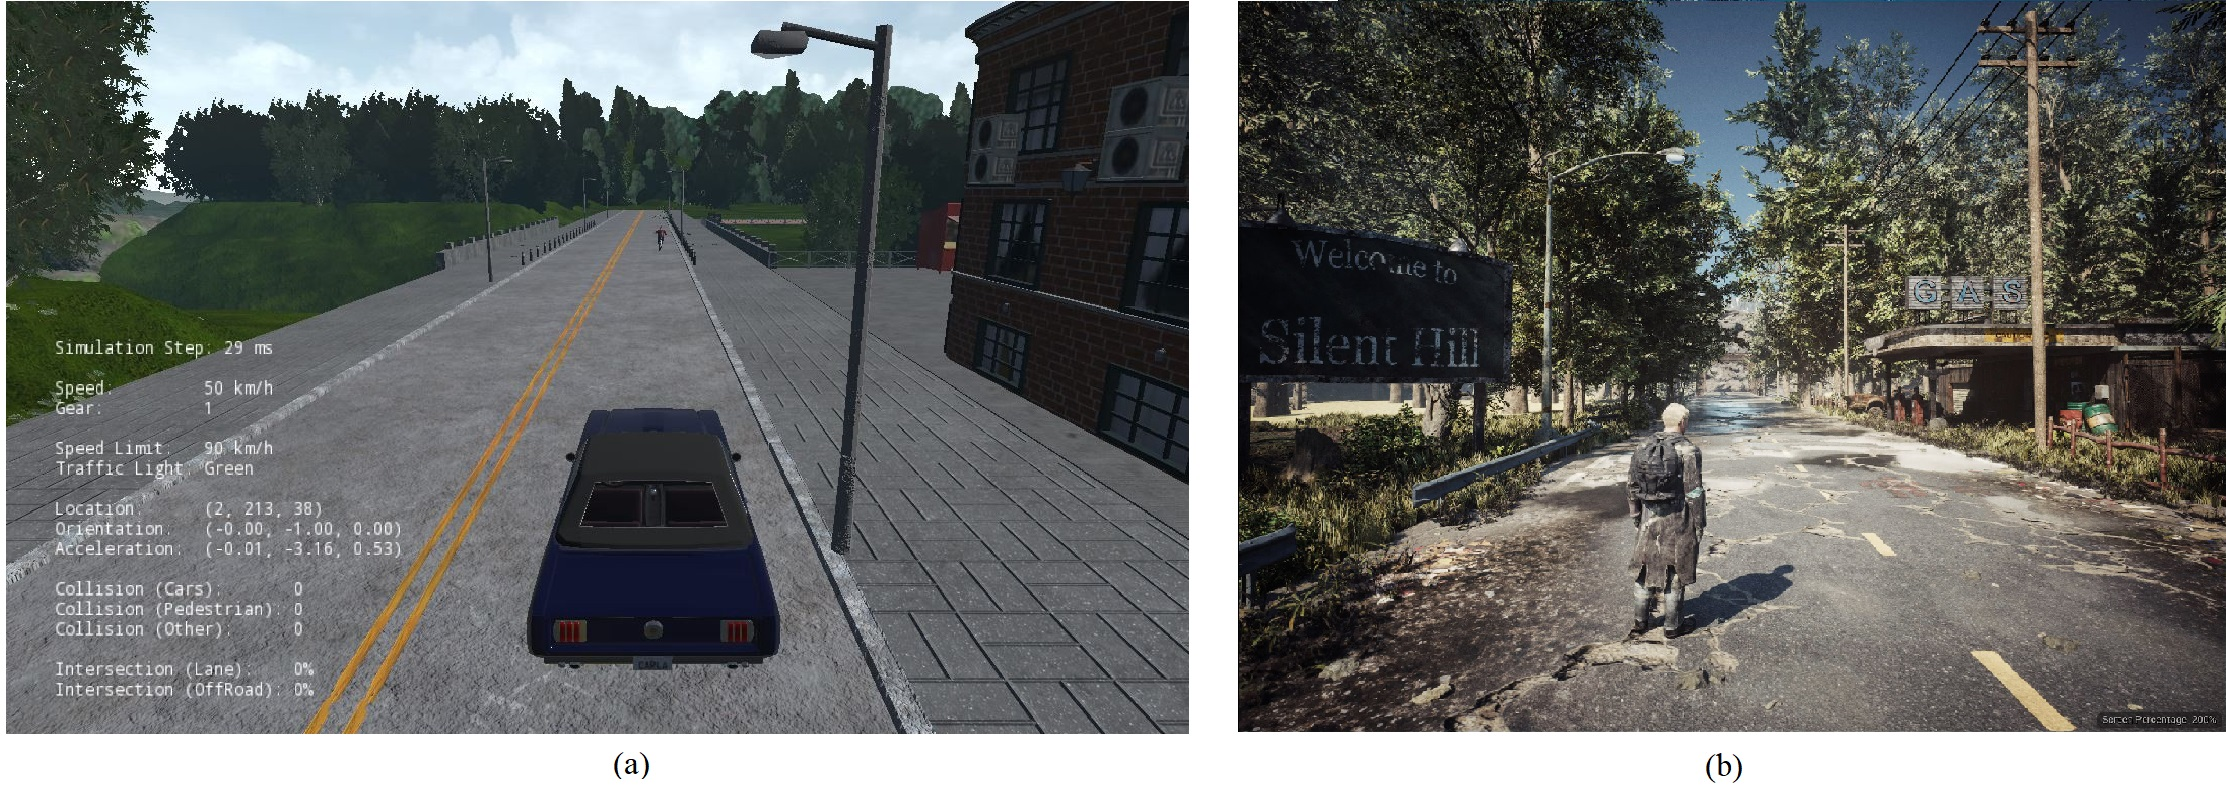
\includegraphics[width=0.95\textwidth]{images/carla-vs-unreal.jpg}
    \caption{Comparison of the capabilities between two simulators of creating realistic 3D environments: (a) CARLA \cite{Dosovitskiy17}, (b) Unreal Engine \cite{scionti2021unreal5}.}
    \label{fig:carla-vs-unreal}
\end{figure}
    

Across the simulators evaluated in the review, where some support more features than others, Unity and UE not only are capable of performing all functionalities described but are the only ones that provide hyper-realistic renderings. Similarly, the authors missed to consider these two engines themselves as general simulation platforms and only focus on physic-specific simulators. In other words, simulators built on top of Unity or UE such as Airsim or CARLA were evaluated. \textcite{juliani2018unity} recognize that simulators are not all equally capable of providing meaningful challenges to learning systems, where a multitude of factors need to be considered to create a worthwhile benchmark for research. Moreover, they stress that modern game engines are not only powerful tools capable of simulating realistic worlds with sophisticated physics and complex interactions, but also are precisely engineered to be intuitive, easy to use, interactive, and provide cross-platform compatibility. It is therefore also our belief, in line with this publication, that game engines are more appropriate for the development and testing in the foreseeable future of AI research. Finally, we would like to draw attention that with the recent release of Unity Engine 5, as shown in Figure \ref{fig:carla-vs-unreal}, the reality gap between synthetic data and realistic data is not far from being closed. Therefore, Unity and Unreal Engine are of special interest to this masters thesis. These game engines are preferred given their simple interface, mature building blocks, multiplatform capabilities, optimized physics engine, 3D rendering, and powerful environment modelling tools. They also allow integration with Python or C++ scripts, respectively. Finally, both frameworks provide an asset store and an active community of developers who actively contribute through forums and release free or inexpensive plugins, 3D assets, shaders, etc.

% Mujoco is
% Gazebo Simulator is
% ALE is
% source https://interestingengineering.com/how-game-engines-work
% Users regard Unity as one of the easiest game engines due to its simple interface. One of the major features it packs is the fact that it enables develop games for multiple platforms. Using the Unity engine, games can be created for Android, iOS and other phone operating systems, including PC OS.  
% 
% On top of its cross-platform capabilities, the platform has an active community of plugin developers who offer lots of free and inexpensive content to use within the game engine. Some examples of games made with the engine include Temple Run, Rust, and Deus Ex: The Fall. Most noteworthy, their personal package is completely free and includes many tools for beginners and hobbyists. You can take a look at various Unity plans here.



% A game engine lays the software framework to build and create video games. They provide features from animation to artificial intelligence. Game engines are responsible for rendering graphics, collision detection, memory management, and many more options.

% A game engine contains five components: The main game program which contains the game logic; a rendering engine which can be used to generate 3D animated graphics; an audio engine which consists of algorithms which are related to sounds; a physics engine to implement 'physical' laws within the system; and Artificial intelligence, a module designed to be used by software engineers with a specialist designation.


% SOURCE: https://www.studytonight.com/3d-game-engineering-with-unity/game-engine

% Engine is like an integrated development environment, with a readymade suite of visual development tools and reusable software components. It turns the complex task of game development simple, by providing an abstraction laye

% it is a framework that is designed specifically for the construction and development of video games

%  just like any other IDE for any particular language programming.

% INPUNT

% There are many different ways of handling an input from deviuces sycg as niyse ganoead jetyboard touch etc
% , two most commonly used are through: events and polling. polling catches events from input devices and polling catches position values where mouse pointers are etc


% Graphics:
% Graphics in a game decides its fate. 3D graphics are designed using 3D assets, which are developed and designed in external 3D rendering programs like Maya, Blender etc and are then imported into the game engine. Hence a good game engine must support multiple import formats.

% Game engine provides a lot of features like lighting effects, shadow, bump maps, blending animation etc to make the imported asset look real.


% Physics:
% There is a sub-component of the game engine, which is known as Physics Engine. Physics engines are software which allows performing fairly accurate simulation of most of the real-life physical systems like the movement of rigid body 
% Gravity, collision detection, rotation & revolution, speed of objects and other such applications are handled by the physics engine within the game.


% Artificial Intelligence:
% How our character reacts on hitting a wall, or seeing an animal etc can be done easily by building a trer of behaviour nodes, rather than writing complex code.

% Sound:
% Audio and Rendering Engines are a sub-part of the Game engine which are used to control the sound effects and generate 3D animated graphics in your 2D screen.

% Networking
% so you do not have to worry about TCP/UDP traffic, social API integrations etc.

% new
% https://www.studytonight.com/3d-game-engineering-with-unity/game-engine
% https://gamedevacademy.org/unity-vs-unreal/
% https://www.creativebloq.com/advice/unity-vs-unreal-engine-which-game-engine-is-for-you
% https://viscircle.de/unreal-engine-or-unity-which-software-should-gamedeveloper-choose/?lang=en


% \textbf{Unreal Game Engine.}\label{chap:2:unity}
% Unreal Engine (UE) is an open-source, free (for non-commercial use) game engine with  UE allows the development of hyperrealistic scenes and has been in a series of works for robotic simulations and reinforcement learning

% https://sim2realai.github.io/UnrealROX/

% https://www.isi.edu/publications/trpublic/pdfs/isi-tr-714.pdf
% .
% % one of the best game engines for rendering detailed graphics. 
% % Some notable games created with the Unreal Engine include Borderlands 2, Dishonored, Mass Effect 3 and Street Fighter V. Supporters of Unreal Game Engine say it can produce some of the best landscapes in gaming. 
% % 
% The pricing model behind this engine includes a free version with full access. 
% However, Unreal Engine takes a 5 percent royalty for any games made from it.

% Applications in ML.

% While Shah and Taylor might seem an unlikely duo, each brings a vital piece of the simulation puzzle: how to accurately simulate complex environmental scenarios, and how to make the scene work with real-time responses from sensors and machines
% \textbf{Mujoco.}
% % 
% MUJUCO, source: https://culurciello.medium.com/design-your-own-robot-for-learning-research-1ca57fe01d63
% 3D scenes
% You may find a nice environment sometimes in Mujoco format. I used to worry, but now fear not! It is easy to create a “.urdf” file based on a Mujoco environment. For example see this one below:
% % 
% an example environment from Google Research
% Mujoco uses “.xml” files to describe words (environments). One can easily translate this type of files into “.urdf”. For example see this original XML file it was translated to this URDF file. This only contains the desk environment with ability to push buttons and open drawers and sliders. You can add a robot arm as per below.
% Robots
% PyBullet makes it easy to import many pre-configured 3D items, robots and tools. The most preferred import is using “.urdf” files. URDF is a file format from ROS that describes robots and tools.
% % 
% Universal Robots arms
% The best way to create your own robot and environment is to use “.stl” files that can be found in many mechanical tools sites, but an easy repository for robotic arms is ROS industrial. For example a very tipical robot arm used in research and also in manufacturing are the ones from Universal Robots, but also Fanuc, etc. You can usually import robot arms via URDF files as this one here.
% Here is an example of how to create an environment with a UR5 robot arm in OpenAI gym format. You can load robot arm URDF together with other desks and furniture, machine and tools in the same way.
% Actuators and Sensors
% When I was using the UR5 robot I was never able to find an easy to use gripper that is easy to implement in PyBullet. A great gripper example I liked is the Mujoco gripper from this environment. I did not dare attempt to create one myself, so I spent a lot of time trying to use the Robotiq 85 or similar, but was always difficult to operate and use. The reason is that it has complex actuation and difficult operation to implement in a gym environment.

% Applications in ML.

% \textbf{Gazebo.}

% Applications in ML.

% \textbf{Arcade Learning Environment.}

% Applications in ML.

For further analysis on landscape simulators, environments and platforms, refer to \cite{collins2021review, juliani2018unity}. 


\subsection{Synthetic Data}\label{chap2:synthetic-data}
Since the quality of a data set distribution can have a negative influence on the quality of an algorithm's prediction and generalization ability, it is important to analyze the quality of the dataset. 
Accordingly, it is claimed that data quality represents 80 percent of the work on AI \cite{8_andrews_2021}, making it important to exploit techniques that allow us to create quality datasets. In general, a data set with an similar number of examples per class can be considered to be a data set with good distributional quality.
% and a data set with a large number of examples per class can be considered to be a data set with bad distributional quality. 
% Techniques that aid in the fabrication of quality datasets ... data augmentation
A technique that enables an alternative method in the creation of quality data sets is synthetic data fabrication.
% Given that the quality of the data set distribution is a critical and deterministic factor for the quality of the predictions in an algorithm,  it is important to analyze the quality of the dataset used by each algorithm. A big help is provided by
% 
% Given the aforementioned descriptions of what makes a 3D environment, it is now important to stress out the importance of the data used in any algorithm. 
% 
%  The distributional quality is influenced by the algorithm which is used and the choice of the data set. However, it is hard to define a criterion that is independent of the data set and its quality, and hence a general criterion that is valid for all data sets.
% 
\begin{figure}[!ht]
    \centering
    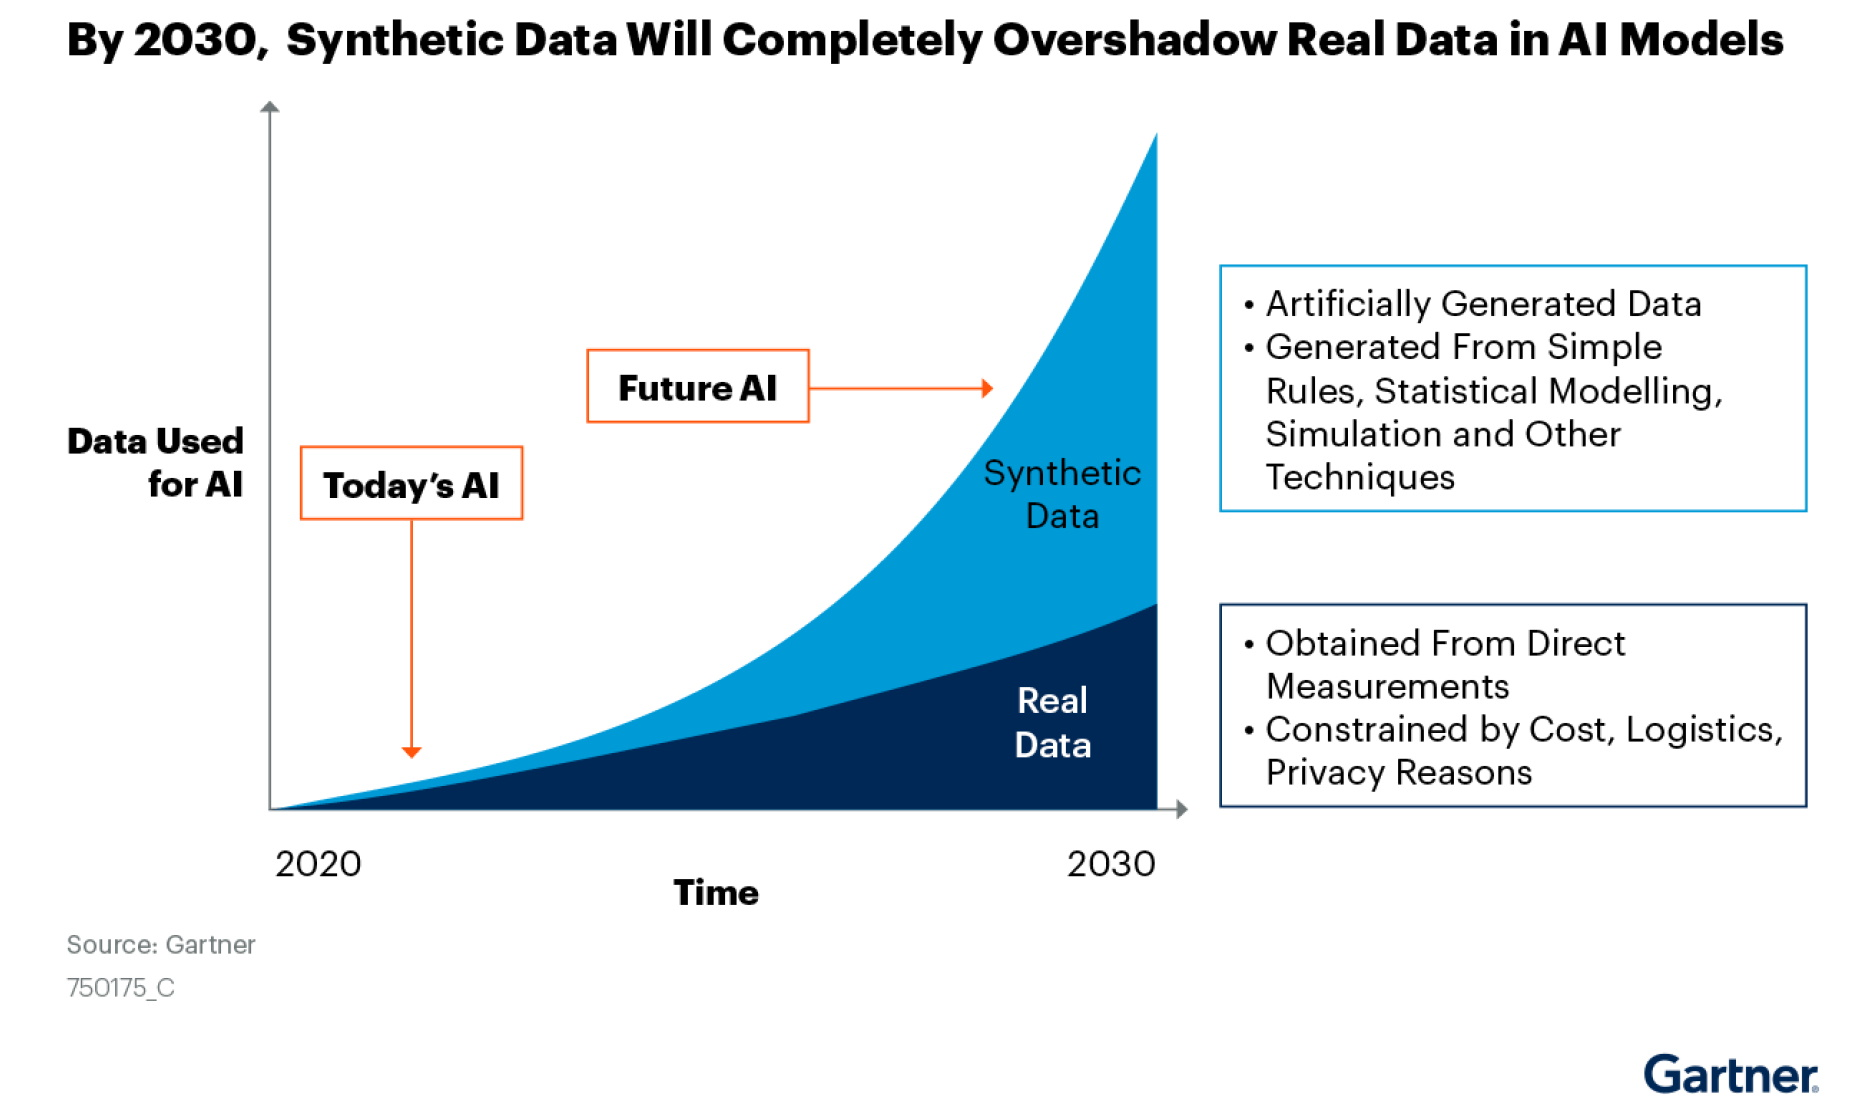
\includegraphics[width=0.75\textwidth]{images/synthetic-gartner.jpg}
    \caption{Synthetic data will become the main form of data used in AI \cite{gartner_inc2021synthetic}.
    }
    \label{fig:synthetic-data}
\end{figure}
    
Synthetic data is generated through simulations, algorithms, or computers, making the results independent of the experimenter. 
% A motivation for synthetic data is the 
A big misconception is that synthetic data can create a skewed image of scientific reality. This concern does not take into account, however, that data synthesis may have the potential to make scientific efforts more efficient. Data synthesis makes the research process more objective by providing a common ground for comparison and allowing experiments to be repeated, such as benchmarks. Additionally, synthetic data can improve the efficiency of experiments because the creation of the data does not have to be done repeatedly. Finally, synthetic data can also prevent researchers from falling into the trap of data dredging, which is when the researcher tests multiple hypotheses using a single dataset. In a June 2021 report on synthetic data\cite{gartner_inc2021synthetic}, Gartner predicted by 2030 most of the data used in AI will be artificially generated by rules, statistical models, simulations, or other techniques. This goes in conjunction and is supported by the breath-taking improvements in Unreal Engine 5's rendering pipeline \cite{unreal5_2021} to develop hyper-realistic 3D worlds, and the innovative advancements shown by Adobe in the past months (2020-2021) through their 3D Substance product line. Adobe 3D Substance includes thousands of models, textures, lighting systems, and uses artificial intelligence to reduce the technical complexity in 3D design and modelling \cite{adobe2021creative3D}. Synthetic data generation is not only a cost-saving technique but it can also sometimes even be better than real-world data, since it includes rare but critical corner cases in the distribution quality of a dataset. 

\begin{figure}[!ht]
    \centering
    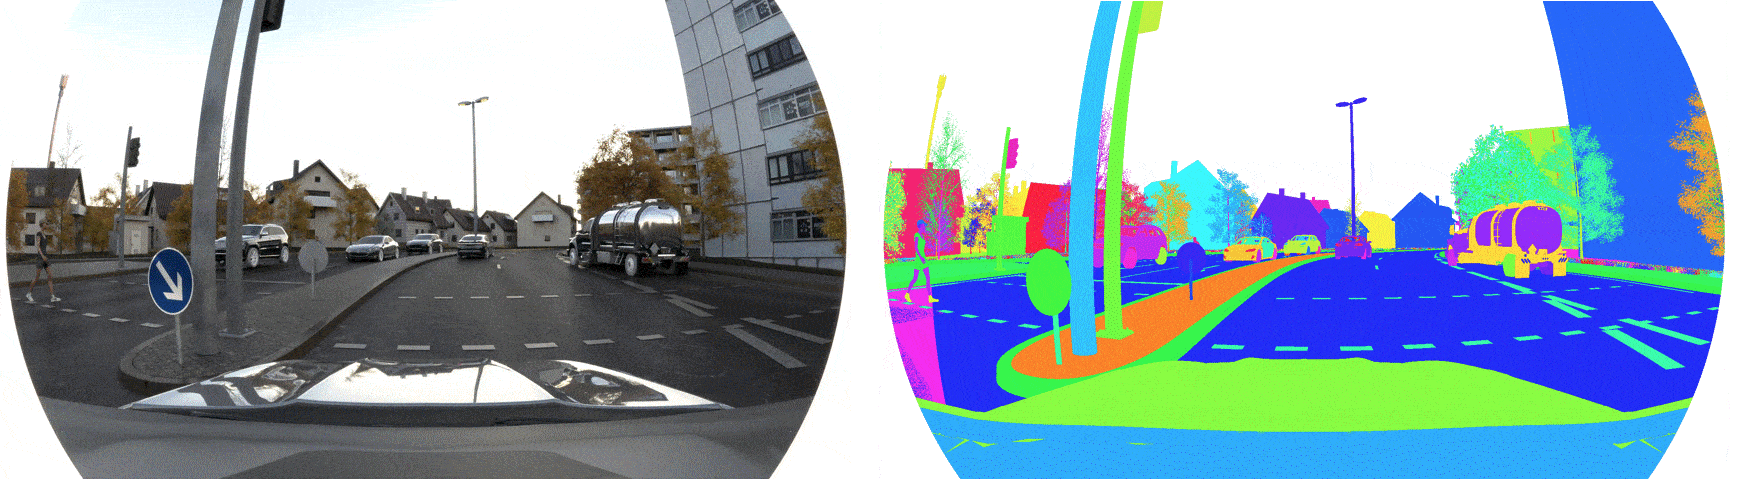
\includegraphics[width=0.95\textwidth]{images/synthetic-data.png}
    \caption{ Developers can alter and randomize objects, colors, lighting, materials and poses in realistic 3D environments to quickly generate synthetic data with perfect labels \cite{8_andrews_2021}.
    }
    \label{fig:synthetic-data}
\end{figure}
    
There are many techniques to generate synthetic data, such as variational autoencoder-decoders algorithms, GANs and simulations \cite{8_andrews_2021}. The factors mentioned in section \ref{chap2:gameengines} that make a good physics simulator such as domain randomization, texture randomization, noise simulation, etc., allow today's game engines to create sophisticated and realistic synthetic datasets, where algorithms and agents can learn more general patterns. Figure \ref{fig:synthetic-data} visualizes how developers and researchers are capable of manipulating 3D environments to generate realistic datasets with extensive domain randomization. It is therefore of special interest in this masters thesis to use the Unity 3D game engine to analyze exploration policies in simulated and realistic environments.
% We do so in three ways: (i) by first measuring the physical characteristics of the environment and the objects within it; (ii) by collecting data in a physical world; and (iii) by generating data in a digital world.


% The objective of this thesis is twofold: Firstly, I will present an implementation of a generative adversarial network that can be applied to create simulated physics based environments in Unity. Secondly, I will investigate how reinforcement learning can be applied to train such generative models in order to generate new data. For this, I will be focusing on the case of an agent that will be trained in the context of the LGP framework.

% The following sections will be organized as follows. In the first chapter, we will briefly discuss what is a generative model, GANs and their implementation in Unity. The second chapter

% https://blogs.nvidia.com/blog/2021/06/08/what-is-synthetic-data/
% https://searchcio.techtarget.com/definition/synthetic-data
% https://research.aimultiple.com/synthetic-data/


